\scanpage{135}

Théorème de \handwritten{- - - - - -} (rapporté par Husemöller).

Soit $A$ une bialgèbre sur le corps $k$, $A$ associative et unitaire pour ses deux structures, ``cocomplète'' pour sa filtration canonique de comodule (duale de la filtration par les puissances de l'idéal d'augmentation du dual; de façon précise, écrivant $\overset{n}{\otimes}A=\overset{n}{\otimes}A^{\handwritten{+}}+$ fo\rlap{r}u\uline{r}bis, d'où via la m.ème itéré\deleted{e} du morphisme diagonal, une application $A\handwritten{\longrightarrow}\overset{n}{\otimes}I^{\handwritten{+}}$, dont le noyau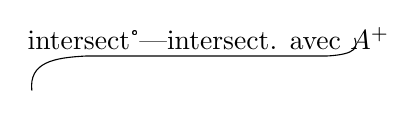
\begin{tikzpicture}[baseline=-.6ex,x=1cm,y=1cm]
\node[anchor=west,inner sep=0] at (0,.42) {\inserted{\handwritten{\unsure{intersect°|intersect.} avec $A^{+}$}}};
\draw (.06,-.24) .. controls (.02,.12) and (.34,.18) .. (.75,.2) -- (3.8,.2) .. controls (4.2,.22) and (4.2,.32) .. (4.16,.43);
\end{tikzpicture} est $\mathrm{Filt}_{m}(A)$).\margin{\handwritten{cela entraine qu'il y a un antipodisme ?}} (NB l'hypothèse cocomplète est satisfaite pour une coalgèbre \inserted{avec unité} à degrés $\handwritten{\geq}$ $0$ réduite à $k$ en degré\deleted{s} $0$, associative et unitaire, - parait-il !). Soit $M$ un $A$-module, muni d'un homomorphisme diagonal 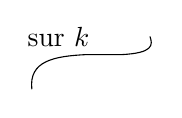
\begin{tikzpicture}[baseline=-.6ex,x=1cm,y=1cm]
\node[anchor=west,inner sep=0] at (0,.42) {\inserted{sur $k$}};
\draw (.06,-.24) .. controls (.02,.12) and (.34,.18) .. (.75,.2) -- (1.2,.2) .. controls (1.6,.22) and (1.6,.32) .. (1.56,.43);
\end{tikzpicture} unitaire (peut-être pas associatif), $M\handwritten{\longrightarrow}M\otimes_{k}M$, qui soit $A$-linéaire,\margin{\figure{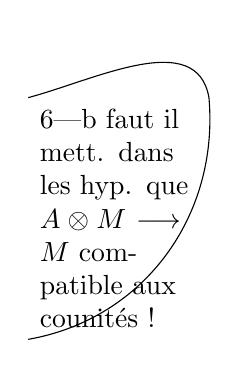
\begin{tikzpicture}
\node[text width=2cm,inner sep=4pt] (n) {\handwritten{\unsure{6|b} faut il mett. dans les hyp. que $A\otimes M\longrightarrow M$ compatible aux counités !}};
\draw (n.north west) to[out=15,in=100] (n.north east) to[out=-85,in=10] (n.south west);
\end{tikzpicture}}}\inserted{\handwritten{(pour la structure de $A$-module sur $M\unsure{\ominus|\otimes}M$ provenant de $A\longrightarrow A\unsure{\otimes|\ominus}A$; il revient au même de dire que $A\unsure{\ominus|\otimes}M\longrightarrow M$ comp. avec application diagonale)}} Supposons de plus donné une ``unité'' i.e. un homomorphisme $k\handwritten{\longrightarrow}M$ qui soit un homomorphisme de coalgèbres unitaires, i.e. $\underset{M}{\mathrm{l}}$'image 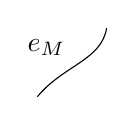
\begin{tikzpicture}[baseline=-.6ex,x=1cm,y=1cm]
\node[anchor=west,inner sep=0] at (0,.42) {\inserted{$e_M$}};
\draw (.13,-.2) .. controls (.46,.2) and (.94,.26) .. (1.01,.67);
\end{tikzpicture} de $1$ satisfait $\handwritten{\epsilon}_{M}(e_{M})=1$, $\handwritten{\Delta}_{M}(e_{M})=e_{M}\otimes e_{M}$. Supposons également $M$ cocomplète, et qu\unsure{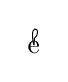
\begin{tikzpicture}[baseline=(e.base),x=1em,y=1em]
\node[inner sep=0] (e) at (0,0) {e};
\draw[line width=.35pt] (0,.1) .. controls (-.06,.28) and (-.08,.65) .. (.03,.67) .. controls (.2,.7) and (.14,.39) .. (.02,.34) -- (.01,.08);
\end{tikzpicture}}\deleted{on} l'application $u\handwritten{\mapsto}u.e$ de $A$ dans $M$ soit injective. Alors $M$ est un $A$-module libre, 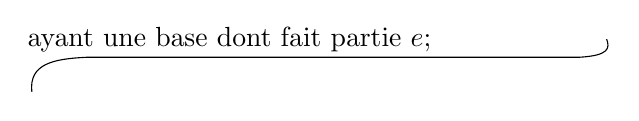
\begin{tikzpicture}[baseline=-.6ex,x=1cm,y=1cm]
\node[anchor=west,inner sep=0] at (0,.42) {\inserted{\handwritten{ayant une base dont fait partie $e$;}}};
\draw (.06,-.24) .. controls (.02,.12) and (.34,.18) .. (.75,.2) -- (7.0,.2) .. controls (7.4,.22) and (7.4,.32) .. (7.36,.43);
\end{tikzpicture} de façon plus précise, posant $\overset{\handwritten{-}}{M}=M\otimes_{A}k$, il existe un isomorphisme (non canonique ...) de $A$-modules $M\handwritten{\overset{\sim}{\unsure{\longleftarrow|\longleftrightarrow}}}A\otimes_{k}\overset{\handwritten{-}}{M}$\handwritten{, tel que le diagramme}
\margin{\handwritten{?}}
\handwritten{\diagram{\begin{tikzcd}[ampersand replacement=\&,column sep=small,row sep=small]
M \arrow[dr] \& \unsure{A|\mathcal{A}}\otimes_{k}\overline{M} \arrow[l,"\sim"'] \arrow[d] \\
\& \overline{M}
\end{tikzcd}}}
\handwritten{commute, et que ...}

Exemple \handwritten{1}. Supposons l'application diagonale de $A$ commutative. Alors $A$ peut être considéré comme l'hyperalgèbre d'un groupe formel connexe 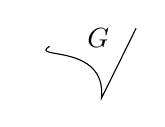
\begin{tikzpicture}[baseline=-.6ex,x=1cm,y=1cm]
\node[inner sep=0] at (.54,.52) {\inserted{$G$}};
\draw (-.08,.42) .. controls (-.35,.25) and (.65,.47) .. (.58,-.24) -- (1.02,.65);
\end{tikzpicture} sur $k$. Si $\handwritten{\Delta}_{M}$ est associatif et commutatif, $M$ aussi est formé des distributions à l'origine d'une variété formelle connexe 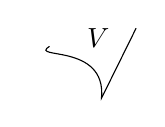
\begin{tikzpicture}[baseline=-.6ex,x=1cm,y=1cm]
\node[inner sep=0] at (.54,.52) {\inserted{$V$}};
\draw (-.08,.42) .. controls (-.35,.25) and (.65,.47) .. (.58,-.24) -- (1.02,.65);
\end{tikzpicture} sur $k$, et le fait que $A$ opère sur $M$ de façon que l'application diagonale soit $A$-linéaire signifie que $G$ opère sur $V$. On voit donc que si $u\handwritten{\unsure{\vdash|\mapsto}}\rlap{\(U\)}u.e$ 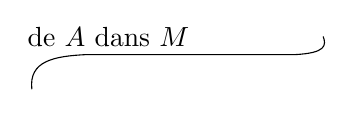
\begin{tikzpicture}[baseline=-.6ex,x=1cm,y=1cm]
\node[anchor=west,inner sep=0] at (0,.42) {\inserted{de $A$ dans $M$}};
\draw (.06,-.24) .. controls (.02,.12) and (.34,.18) .. (.75,.2) -- (3.4,.2) .. controls (3.8,.22) and (3.8,.32) .. (3.76,.43);
\end{tikzpicture} est injectif, i.e. si $g\handwritten{\mapsto}g.a$ ($a$ le \handwritten{``}centre\handwritten{''} de $V$) de $G$ dans $V$ est un monomorphisme, alors $M$ est libre sur $A$. En fait, on trouvera que $G$ opère librement sur $V$ i.e.
% archive sheet number: 134
